\section{Background}

\subsection{ProB 2.0}

ProB is written in primarily in SICStus prolog \cite{LeBu08_225}. This core is packaged as a binary executable command line interface, and several other tools have been built on top of it to provide the user with a functioning user interface. The user interface for the current standalone ProB application is written in Tcl/Tk. It is in this application that the GraphViz rendering engine has been integrated. 

ProB 2.0 is another tool that is built on top of the ProB command line interface. It is the successor of an Eclipse RCP plugin that has been in development since 2005 \cite{BuHa07_292}. This application was created so that ProB could be integrated with the Rodin software, which is an easy to use and extensible tool platform for editing specifications written in the Event-B specification language.

In 2011, development for ProB 2.0 began. The main goal of ProB 2.0 was to adapt and optimize the existing Java application to produce a programmatic API. One of the main improvements made available in this tool was the introduction of a programmatic abstraction of the state space. It also provides a programmatic abstraction for the represenation of animations. This abstraction consists of the trace of transitions that have been executed during the course of an animation. This also provides the user with the concept of a current state. ProB 2.0 also contains a listener framework that is triggered whenever changes take place within a state space or within an animation.

The core harnesses the power of the Groovy programming language. It integrates integrates a fully functioning groovy console into the final product. It is now possible for users and developers to write Groovy scripts that carry out desired functionality. There is also support for creating web applications that communicate with ProB. The console is actually a user interface that makes use of the jetty server that is integrated in the ProB 2.0. There are no eclipse dependencies present in the core, so it can be deployed as a jar file and integrated into any Java based application.

ProB 2.0 also contains an Eclipse RCP Plugin that builds on top of the programmatic core and provides the interface with which the application can communicate with the Rodin platform. The graphical user interface is now built on top of the new programmatic abstractions that are available from the core, and changes that take place within the graphical interface are triggered by the listener framework.

The visualizations that we have created in the course of this work are integrated into ProB 2.0. They pure JavaScript applications that communicate with Java servlets responsible for generating the data that needs to be visualized. Within the Eclipse user interface, they are simply loaded into a browser.

\subsection{D3 and JavaScript}

Since a jetty server was already available in the ProB 2.0 Plugin, it was plausible to create visualizations using javascript and HTML. Because the ProB 2.0 Plugin is an Eclipse application, it also would have been possible to create visualizations using a native Java or Eclipse library. I carried out an experiment at the beginning of this work to determine the feasibility of the different graph libraries. JUNG was considered because it is the software framework that is the ProB 2.0 API currently uses. It would have been relatively simple to embed the visualizations into the existing ProB 2.0 Plugin, but customizing JUNG graphs is extremely difficult. The ZEST graph library was a feasible option, but in the end, I chose to use the D3 library. 

D3 (Data-Driven Documents) is ``an embedded domain-specific language for transforming
the document object model based on data'' which is written in JavaScript \cite{2011-d3}. Developers can embed the library into a JavaScript application and use the D3 functions to create a pure SVG and HTML document object model (DOM). The focus of D3 is not on creating data visualizations. It is on providing the user the capability of defining exactly which elements the DOM should contain based on the data that the user has provided. Because the objects that are being manipulated are pure SVG and HTML, the user can use D3 to create objects that can be styled using CSS or by dynamically manipulating the style tags of the elements.

\subsubsection{Core Functionality}

D3 provides a selector API based on CSS3 that is similar to jQuery\footnote{http://jquery.com}. The user creates visualizations by selecting sections of the document and binding them to user provided data in the form of an array of arbitrary values \cite{2011-d3}. D3 provides support for parsing JSON, XML, HTML, CSV, and TSV files. Once the data is bound to the desired section of the document, D3 can append an HTML or SVG element onto the section for each element of data. This is where the real power of D3 lies because the user can define the attributes of the element dynamically based on the values of the datum in question. By changing these attributes (e.g. size, radius, color) the resulting document already presents the data in a way that the viewer visually understands. The core also provides support for working with arrays and for defining transitions that can be used to animate the document. In order to better understand how D3 works, we have provided a simple example of a how a developer can use D3 to create an HTML dropdown menu (see Listing \ref{d3Example}). The generated HTML snippet is also provided (see Listing \ref{d3Result}). A more complicated example using the force layout is available in the appendix (see Appendix \ref{appendix:force}).

\subsubsection{Further Functionality}

D3 also provides further functionality for manipulating the DOM. Developers can define a scale based on the domain and range of values that are defined in the data provided by the user. The placement of elements within the document can then be placed according to the desired scale. D3 provides support for many different types of scales including linear scales, power scales, logarithmic scales, and temporal scales. Axes can also be created to correspond to the defined scale.

The user has the ability to change the DOM as needed. However, D3 also supports a large number of visualization layouts so that the user does not have to define the positions for the elements in a given visualization. The two layouts that are of relevance for this work are the tree layout and the spring layout.

The tree layout uses the Rheingold-Tilford algorithm for drawing tidy trees \cite{Reingold81}. The force layout uses an algorithm created by Dwyer \cite{Dwyer2009} to create a scalable and constrained graph layout. The physical simulations are based on the work by Jakobsen \cite{Jakobsen03}. The implementation ``uses a quadtree to accelerate charge interaction using the Barnes–Hut approximation. In addition to the repulsive charge force, a pseudo-gravity force keeps nodes centered in the visible area and avoids expulsion of disconnected subgraphs, while links are fixed-distance geometric constraints. Additional custom forces and constraints may be applied on the ``tick'' event, simply by updating the x and y attributes of nodes'' \cite{D3Wiki}.

To help the viewer interact with the visualization, D3 provides support for the zoom and drag behaviors. This listens to the mouse clicks commonly associated with zooming (i.e. scrolling, double clicking) and enlarges the image as would be expected. With this same mechanism, the developer can enable the user to grab hold of the canvas and pan through the image to inspect it closer.

Despite the considerable functions that D3 offers, it is very easy for the user to begin developing with D3. The API is described in detail on the D3 Wiki \cite{D3Wiki}, and the D3 website\footnote{http://d3js.org} includes an extensive array of examples that new developers can use as a jumping off point. The D3 developer community is very large, so it is easy to find answers to almost every question online. 

\lstset{language=Java}
\begin{lstlisting}[caption=Dynamically create a dropdown menu.,label=d3Example]
// Select element with id "body" and append a select tag onto it. When it changes, the defined function will be triggered.
var dropdown = d3.select("#body")
				   	.append("select")
				   	.on("change", function() {
				   		var choice = this.options[this.selectedIndex].__data__;
				   		// handle choice
				   	});

var options = [{id: 1, name: "Option 1"},
			   {id: 2, name: "Option 2"},
			   {id: 3, name: "Option 3"}];

// Create an option tag with id and text elements for each option that is defined in options
dropdown.selectAll("option")
		.data(options)
		.enter()
		.append("option")
		.attr("id", function(d) { return "op" + d.id; })
		.text( function(d) { return d.name; });

// Select option 3 by default
dropdown.select("#op3")
		.attr("selected", true);
\end{lstlisting} 

\lstset{language=HTML}
\begin{lstlisting}[caption=Html generated from Listing \ref{d3Example},label=d3Result]
<div id=body>
    <select>
        <option id="op1">Option 1</option>
        <option id="op2">Option 2</option>
        <option id="op3" selected=true>Option 3</option>
    </select>
</div>
\end{lstlisting}


\subsection{GraphViz integration with emscripten}

The current visualizations available in the ProB Tcl/Tk application are powered using the GraphViz\footnote{http://www.graphviz.org} graph visualization software. In the ProB CLI, there is support for generating graphs for the state space in the DOT graph language. The problem with this, and the reason that we are researching other alternatives, is that drawing GraphViz graphs is extremely inefficient. However, for the state spaces that are derived using the signature merge algorithm, or for the transition diagrams that can be created from a state space, these graphs are quite pleasing to the eye. The derived graphs are also usually small enough that they can be drawn efficiently.

For this reason, we wanted to some how be able to visualize small graphs written in the DOT language. In order to do this, we took advantage of the emscripten compiler \cite{emscripten}. This is a compiler that compiles LLVM bitcode to JavaScript so that it can be run in any browser. Any C programs can be compiled to LLVM. We used the Viz.js JavaScript library\footnote{https://github.com/mdaines/viz.js} developed by Mike Daines which has compiled GraphViz from C to JavaScript and provided a wrapper function to produce svg visualizations. For example, the code shown in Listing \ref{vizJs} will produce Figure \ref{graphVizEx}.

\begin{lstlisting}[caption=Create a visualization with viz.js and insert it into an html page.,label=vizJs]
svg = Viz("digraph { a -> b; a -> c; }", "svg");
$("#elementId").replaceWith(svg);
\end{lstlisting}

\begin{center}
\begin{figure}[h!]
\centering
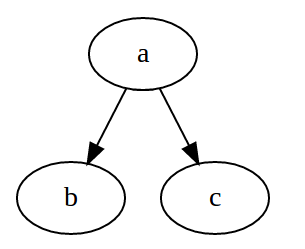
\includegraphics[width=8cm]{bilder/graphVizExample.png}
\caption{Generated graph image from Listing \ref{vizJs}.}
\label{graphVizEx}
\end{figure}
\end{center}